%!TEX root=writeup.tex

\section{Natural Language Based CLI Framework}

\begin{figure}[h]
    \begin{center} 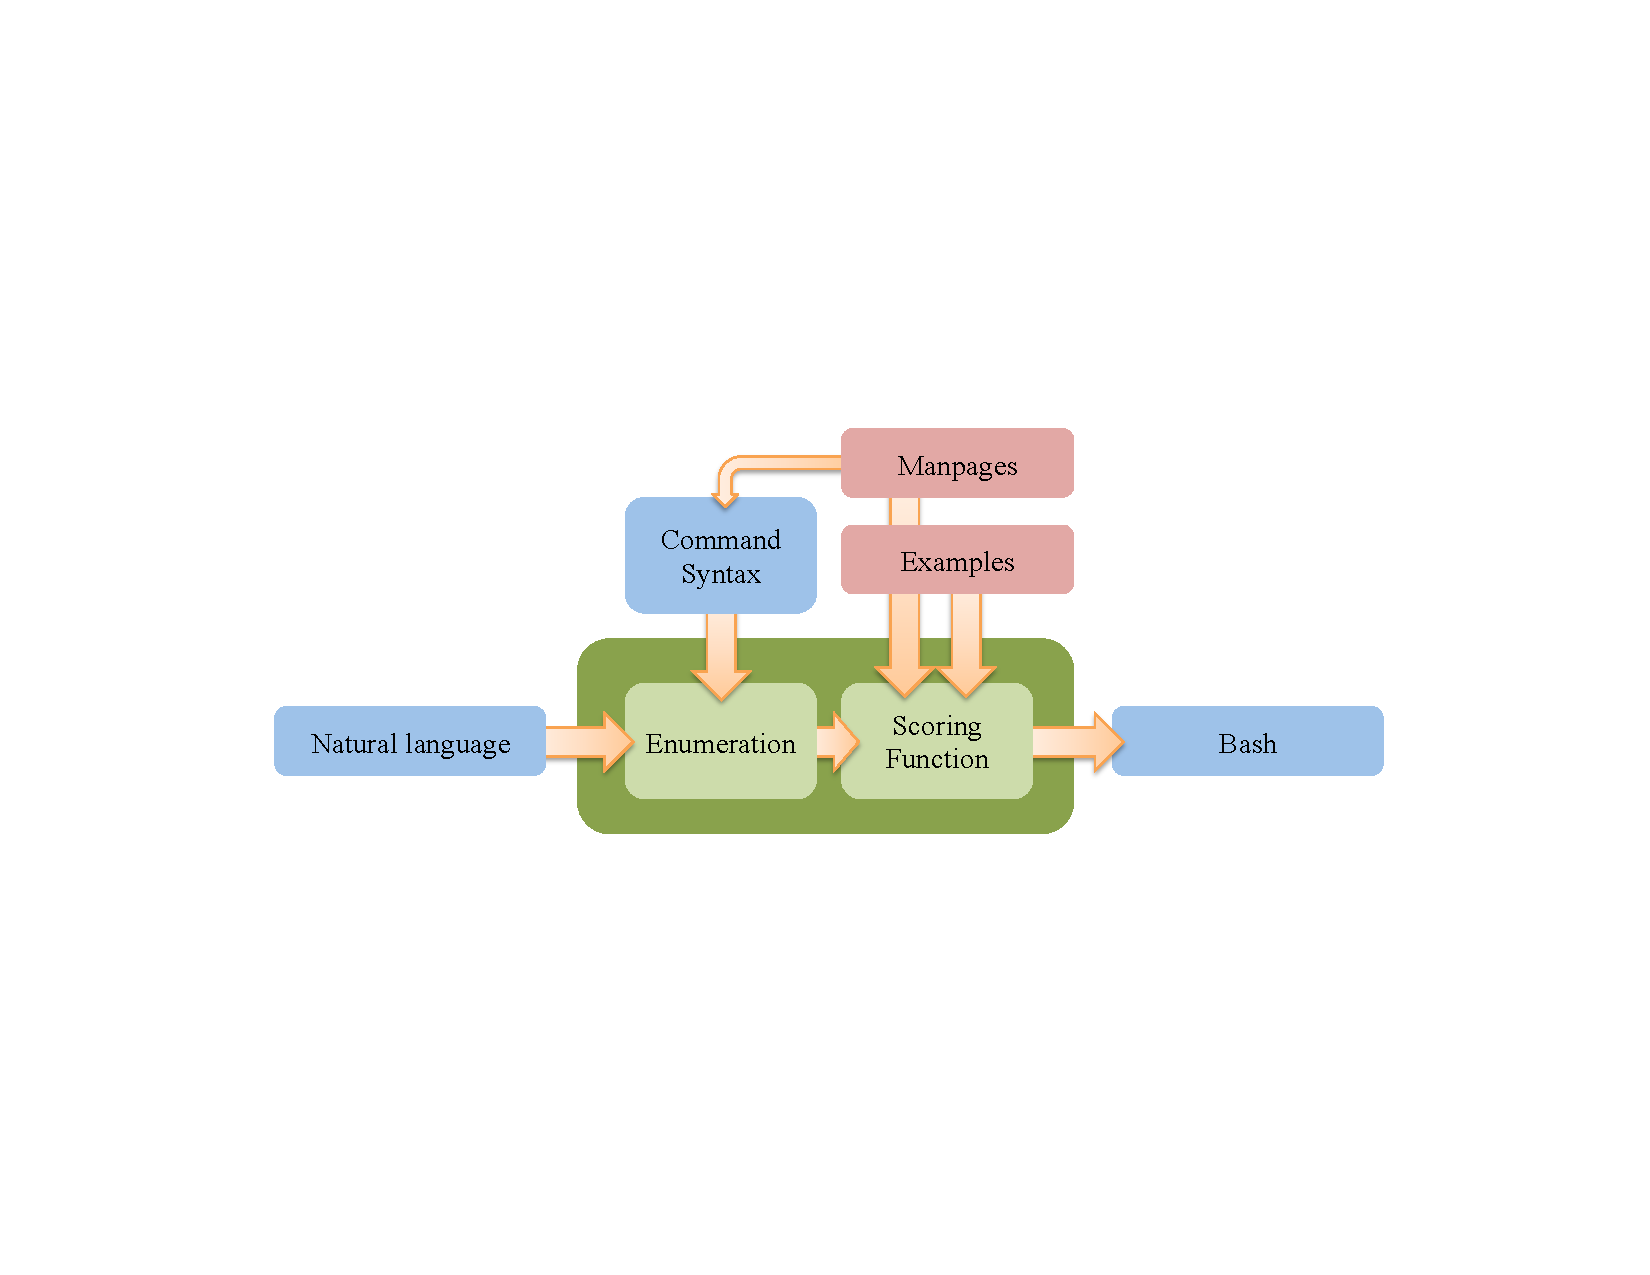
\includegraphics[width=4in]{architecture.pdf} \end{center}
    \caption{The overall architecture of our tool. Offline, the tool learns the
        valid syntax for common Bash commands using manpages. Both the manpages
        and a set of input-output examples are used to learn an appropriate
        scoring function. At runtime, the tool enumerates possible candidate
        programs using the learned syntax, scores them using the learned scoring
        function, and presents the top-ranked suggestions to the user.}
    \label{fig:arch}
\end{figure}

The natural language based command line interpreter we plan to develop consists of three key components: 1) an intermediate logic representation based on which Linux commands are generated, 2) a learnig algorithm that can extend basic operations of the intermediate language with provided natural language manuscript and 3) a semantic parser that effectively maps the natural language commands issued by users to this intermediate representation. Especially, our initial pilot system is restricted to cover only file system operations, including file lookup, directory tree transformation, file content transformation, file property modifications. We restrict the domain in the hope that it can be expressed with tractable logic as well as to reduce the degree of ambiguity in the natural language command.

\subsection{Intermediate Representation of File Operations}
\label{subsec:represent}
Our ideal intermediate representation is one based on which the executable commands can be deterministically generated, but is also reasonably similar to natural language semantics such that an accurate translation is not beyond hope.
\paragraph{Representation of File System}
We plan to represent the file system as a tree, such that leaf nodes represent regular files and others are directories. Properties and file contents are represented as attributes of node. With this presentation, we can reduce the file system manipulation problem to tree transformation problem.
\paragraph{Representation of File Operations}
File operations contains 1) structural transformation operations and 2) basic CLI operations. The first set of operations are designed to perform tree structure transformation, and they are used to hide lower-level command line program implementations. While the second are basic operations related to file property lookup (e.g. lookup the access date of a file).

Since the number of basic Linux commands and options is large even in domain-specific scenarios, it is difficult for a human designer to hand-code all of the generation rules. We plan to semi-automate this step by adding information extracted from the Linux man pages\footnote{\url{http://linux.die.net/man/}} and make the language extensible.

\subsection{Natural Language Command Interpreter}
We plan to train the natural language command interpreter in a supervised setting, assuming a set of natural language and Linux command pairs are available. The intermediate logic representation, however, remains as latent variables in our model. We score a natural language to logical representation mapping based on the following features:
\begin{itemize}\itemsep-1pt
	\item association of key words/phrases to partial logical formulas
	\item association between partial logical formulas (e.g. how often do they combined in valid commands)
	\item if the ground truth command can be generated from the logic representation
	\item complexity of the logical formulas and the commands generated from them.
\end{itemize}
The weights of these features are learned using the training set. We planned to extend learning into an interactive setting once the basic framework is developed.